%!TEX root = vaisagh_thesis.tex

\chapter{Modelling Pre-evacuation Behavior}
\label{chapter:PreEvacuationBehavior}


Ideally, when a fire starts a fire alarm goes off; all occupants hear this alarm and use the nearest safe exit to leave the building. However, this is hardly the norm. In many cases, occupants are desensitized from hearing false alarms and often do not start to evacuate until they are completely sure that egress is necessary. On January 19, 2000, a fire in Boland Hall in Seton Hall University killed three students because they had ignored the fire alarms assuming they were false~\cite{Berry:2000us}. This uncertainty about the authenticity of the first sign of danger isn't an isolated incident~\cite{Graham:2000vl,Proulx:2001we,Proulx:1995wq,Proulx:2003tc,Purser:2001ts,Ramachandran:1990wj,Sime:1995uu,Tong:1985wn}. This delay in reaction time of evacuees can have a huge impact on existing plans for egress if it is not taken into consideration. Thus, it is important to consider this when developing evacuation plans. In other words, when studying the behavior of evacuees, it is necessary to study and understand their actions from the time at which the fire started right up until the point where the last person evacuated~\cite{Tong:1985wn}.



As discussed in Chapters~\ref{chapter:LiteratureReview} and~\ref{chapter:IBEVAC}, pre-evacuation uncertainty and investigation are features of human behavior during egress that are rarely considered in existing models. To recap, \emph{pre-evacuation} refers to the period of time that elapses after the start of the fire alarm before the person starts evacuating. While some models~\cite{Tsai:2011tz} do have a simplified model of pre-evacuation behavior, they fail to model it in enough detail to enable their extension to more general cases. For example, a fire alarm could have different effects based on the clarity and believability of the alarm~\cite{Kobes:2009jx,Paulsen:1984ti}. This variability is hard to simulate in existing models of pre-evacuation behavior. Also, during an evacuation people exchange event and environment related information with others. Evacuees are unlikely to follow every message that they receive blindly. There is a variability in the \emph{trust} in messages received that can have different effects on egress. This is rarely considered in existing models.


In this chapter, we present a model for simulating pre-evacuation behavior and event identification\footnote{This model was presented at the Pedestrian and Evacuation Dynamics Conference in 2012 and appeared in print in 2014~\cite{Viswanathan:2012vt}.}. In the model, the evacuees identify and process information in terms of event cues which exist throughout the environment. Section~\ref{PreEvac:LitRev} first explores some of the existing work that motivates the need to model pre-evacuation behavior. Following this, Section~\ref{PreEvac:EventIdentification} explains the proposed model and, finally, Section~\ref{PreEvac:Results} illustrates through experimentation the usefulness of this model, the importance of modelling pre-evacuation behavior and having a communication model.



\section{Related Work}
\label{PreEvac:LitRev}


As discussed in Section~\ref{LiteratureReview:CurrentUnderstanding}, there are a lot of conflicting theories on how humans behave in emergencies and why they behave as they do. However, there are certain behaviors that are fundamental to human nature and are generally accepted as fact, such as the constant search for information~\cite{Proulx:2003tc,Tong:1985wn,Ozel:2001tn,Sime:1983uy}. This section first summarizes the existing knowledge of human behavior during egress with special emphasis on pre-evacuation behavior. Following this, some existing models of pre-evacuation behavior and evacuee communication are presented.

\subsection{On modelling pre-evacuation behavior}
\label{PreEvac:PreEvacuationBehavior}

Several studies of human behavior during emergency egress~\cite{Kuligowski:2005tt,Ozel:2001tn,Proulx:2007ul}, have shown that an evacuee's first reaction after realizing that there is an unusual situation is to investigate and gather more information about the situation. Evacuation starts only once the need for evacuation is established. \emph{Cues} are the key to understanding this transition from realization to investigation and, eventually, to evacuation.

Cues are certain changes in the environment that indicate that something is wrong or different from normal~\cite{Sime:1983uy}.
They come in different forms. Fire and smoke are the typical and most effective cues for an evacuation. Fire alarms and people running or instructing to escape are also cues. According to Sime~\cite{Sime:1983uy}, there are three kinds of cues:
\begin{itemize}
\item Ambiguous Cues: E.g. Hearing noises or shouting, or seeing someone run.
\item Verbal Cues: E.g. Instructions from a companion, announcement from the stage.
\item Unambiguous Cues: E.g. Seeing smoke or fire, or seeing someone run with a fire extinguisher.
\end{itemize}


According to some researchers~\cite{Ramachandran:1990wj,Proulx:2007ul}, an ambiguous cue by itself does not cause a person to initiate investigation. Rather, the cue has to persist for a period of time before investigation begins and results in the finding of an unambiguous cue. Interestingly, according to Tong and Canter~\cite{Tong:1985wn}, even unambiguous cues don't result in people immediately exiting the building, rather it initiates a complicated process consisting of information searching and affiliation.

The effect of cues and the evacuee's reaction to it depends on many factors. The identity of an individual's primary group and its proximity and availability determines the reaction of a person to a cue~\cite{Sime:1983uy}. In~\cite{Latane:1969wm} an experiment was conducted where particpants were placed in a room with smoke; the experiment showed that when alone, 75 percent of the subjects reported the smoke. However, in the presence of two non-reacting others only 10 percent of the subjects reported the smoke during the experimental period.

Various studies~\cite{Proulx:2003tc,Proulx:2001we,Paulsen:1984ti,Sandberg:1997tw,Cocking:2008vv,Tong:1985wn} emphasize the importance of the location and the person's role in the significance of cues. As an example, a fire alarm at home is more likely to cause a person to act than a fire alarm at their office, which will most likely be considered a false alarm. People's societal role determines their training and responsibility and thus their alertness to cues and the preparedness for reacting to it.

Their groups, location and environment aren't the only factors that influence people's behavior during evacuation. There are also a lot of \emph{intrinsic factors} that influence how people react to fires. What these factors are and how influential they are are a matter of much debate. Over the years there have been several surveys~\cite{Tong:1985wn,Sandberg:1997tw,Kuligowski:2009un} that discuss these intrinsic factors.

Andr\'{e}e and Eriksson's report~\cite{Andree:2008td} even had a cross cultural study that compared the evacuation behavior of Swedish students against the behavior of Australian students. Except for grouping behavior they found few significant differences in the behavior during evacuations. Kobes et al., in their survey~\cite{Kobes:2009jx}, compared some studies of evacuation behavior from the USA, Great Britain and Australia and commented on them being ``identical in their essence''. Some factors like age and gender were found to not significantly affect pre-evacuation behavior. A person's social role is one of the commonly accepted factors that influence evacuation behavior~\cite{Sandberg:1997tw,Kobes:2009jx,Paulsen:1984ti}. Factors like the person's experience with fires, training, disabilities, familiarity with the environment, etc.\ are accepted to have a great influence on pre-evacuation behavior.

Close to a hundred different studies on human behavior in fires were used by Kuligowski~\cite{Kuligowski:2009un} to compile a list of the factors that influence egress and more specifically pre-evacuation behavior. In this article, she suggests that the period that we term as \emph{pre-evacuation} itself consists of two phases. Phase 1 is called \emph{perception}; The idea being that the existence of a cue does not guarantee its perception. The Table~\ref{tab:Cues} lists some factors that can affect this perception of a person and whether these factors increase or decrease the chance of the person perceiving the abnormality in the situation.

Kuligowski calls the next phase \emph{interpretation}. During this phase, the person searches for more information to verify whether a fire has actually started and if it actually poses a threat that needs to be handled. Many studies~\cite{Ozel:2001tn,Proulx:2007ul} have confirmed the importance of this phase, though sometimes they are known by different names. In~\cite{Ozel:2001tn} this phase is called \emph{unconflicted inertia} to indicate how the person either continues what he's doing or tries to finish of his activity without actually beginning to evacuate. In~\cite{Tong:1985wn}, this phase is called \emph{investigation} to indicate the search for information that enables the interpretation of the system. Regardless of what it is called, this phase consists of two parts:
\begin{inparaenum}
\item defining the situation as a fire and
\item defining the risk that the situation poses.
\end{inparaenum}


Kuligowski categorized the factors that influence these phases into two types: occupant based factors~(which are equivalent to the intrinsic factors mentioned earlier) and cue based factors. These factors and their effects are shown in Table~\ref{tab:Cues}. Increases/Decreases signifies a cues effect on that particular phase. Also, cue based factors, do not simply consist of events, but also their nature and features.


% Requires the booktabs if the memoir class is not being used
\begin{table}[htbp]
\centering
\begin{threeparttable}[b]
\topcaption{Factors affecting Evacuation Behavior.] The list of factors affecting evacuation behavior and their influences as presented in Kuligowski's survey~\cite{Kuligowski:2009un}} % requires the topcapt package
\begin{tabular}{m{6.3cm} c >{\centering\arraybackslash}m{2.8cm} >{\centering\arraybackslash}m{2.8cm}} % Column formatting, @{} suppresses leading/trailing space
\toprule
Factors & Perception  & 2a: Definition of the Situation as a Fire & 2b: Definition of the Risk to Self/Others\\

\midrule
\multicolumn {4}{l}{{\bf Occupant-based pre-event factors}}\\
\midrule
Has experience with fires    & Increases  & Increases &  Increases\\
Has knowledge of fire/ training & Increases  & Increases &  Increases\\
Habituation with environment   & Decreases  & ---\tnote{1}    &  --- \\
Has knowledge of routes     &   ---   &  ---    & Decreases\\
Has frequent experience with false alarms & ---  & Decreases &  ---\\
Has a feeling of security in the building & ---  & Decreases &  ---\\
Has perceptual disability   & Decreases  & --- &  ---\\
Is older adult        & Decreases  & --- &  Increases\\
Is woman           & Increases  & --- &  Increases\\
Speaks the same language as others & Increases  & --- &  ---\\
Has frequent interaction with family & Increases  & --- &  ---\\
\midrule
\multicolumn {4}{l}{{\bf Occupant-based event factors}}\\
\midrule
Has a higher stress/ anxiety level  & Decreases & --- & --- \\
Perceives a time pressure & Decreases & Decreases & Increases \\
Presence of others~(especially loved ones) & Decreases & --- & Increases \\
Proximity to fire / Visual Access  & Increases & --- & --- \\
Sleeping & Decreases & ---& ---\\
A higher number of behavioral processes(>1) & --- & Increases & --- \\
Defines situation as a fire & -- & N/A & --- \\
\midrule
\multicolumn {4}{l}{{\bf Cue-based factors}}\\
\midrule
A higher number of cues & Mixed\tnote{2} & Increases & Increases \\
Consistent cues & --- & Increases & Increases \\
Unambiguous cues & --- & Increases & --- \\
Social cues~(others' actions) that are consistent with an understanding of a fire situation & --- & Increases & Increases \\
Official source & Increases & Increases &---\\
Familiar source & --- & Increases &--- \\
A higher dose of toxic gases & --- & Decreases & --- \\
Extreme/ dense cues & Decreases & --- & Increases \\
Visual/ audible cues & Increases & --- & --- \\
Risk Information & --- & Increases & --- \\
\bottomrule
\end{tabular}
\begin{tablenotes}
\item[1]{Areas where no research is found is marked by ---}
\item[2]{Research conflicted on the direction of influence of this factor}
\end{tablenotes}
\label{tab:Cues}
\end{threeparttable}
\end{table}



One of the factors that encourage the programmatic implementation of cue based factors is the fact that the effect of a cue can be explained to be caused by the nature and characteristics of the cue rather than the specific cue. In other words, each cue can be described in terms of its ambiguity, consistency with other cues and its source and it is this description that determines the effect of the cue.


\subsection{Existing models}
\label{PreEvac:ExistingModels}

There are very few existing models that take pre-evacuation period into consideration. Pre-evacuation decision making of an individual was modeled by Pires~\cite{Pires:2005gs} using a simple Bayesian Belief Network~(BBN).

Fran{\c c}a et al.~\cite{Franca:2009wq} created a simulation model of the development of panic behavior during emergency egress. This model implemented the hysterical belief theory~\cite{Torres:2010tj} and modeled how panic first develops and then evacuation happens. It also had a basic communication system through which agents exchanged mood information (which is a key factor in the development of panic) by using the grid based environment as a medium for communicating messages. Despite pre-evacuation behavior being modeled in some detail, it is not possible to extend this model to replicate the heterogeneity in people's reaction to cues.

ESCAPES~\cite{Tsai:2011tz} is a model that takes into account some factors like the spread of knowledge, fear and emotion between the different evacuees. These factors are used to create a simplistic model of pre-evacuation behavior. Effectively though, only the \emph{perception} part of pre-evacuation behavior is modeled. This means that  once an agent perceives a cue i.e. another agent running, the perceiving agent immediately starts to evacuate.

The event identification and communication model proposed in this chapter have been influenced by these models. However, it is unique in the way that the diversity of cues and their effects can be considered; and more importantly, in how both the perception and investigation phase of pre-evacuation behavior can be simulated in this computational model. Data on pre-evacuation behavior is difficult to gather: If participants are given prior warning like in fire drills, their behavior is likely to be unrealistic; on the other hand, not giving prior warning could be risky and dangerous. Thus, in this chapter, the proposed models are validated against established theories.

\section{A Bucket Model of Event Identification}
\label{PreEvac:EventIdentification}

% First explain how cues are modeled
Section~\ref{PreEvac:PreEvacuationBehavior} discussed how ambiguity, source and consistency of the cue~\cite{Kuligowski:2005tt,Sime:1983uy,Tong:1985wn} are the key factors in determining the effect of a cue. This is the fundamental idea used in the proposed model. Ambiguity refers to the clarity of the cue. A cue that gives a clear signal of an event would be unambiguous while an ambiguous cue will lack this clarity. For example, a traditional ringing fire alarm is highly ambiguous while the modern fire alarms with voice updates are much less ambiguous and they have different effects on pre-evacuation behavior. The source of a cue is also important; there is a clear difference in perceived danger in a situation when the warning is given by figure of authority like a fire marshal as opposed to an unknown stranger. Lastly, if the signals given by cues are inconsistent then it would take longer for a person to start egress. For example, if no other occupant is perceived to be raising an alarm or trying to evacuate, most people would not react to smoke~\cite{Latane:1969wm}.

Each cue is located at a particular location $(x,y)$ in the environment and is sensed by agents when within their perception range. When a cue is sensed, an agent obtains a certain amount of information $\mu$ about the current state of the world. Thus, a cue in the Bucket model is represented as a tuple $(\mu, x, y)$ where $\mu$ is the amount of information obtained from the cue and $(x,y)$ is the location of the cue. When an event or an action of significance occurs at some location a cue is created at that location.


Once perceived, these cues are processed by the agent's Event Knowledge System which manages the information from cues. The Event Knowledge System has two \emph{buckets}  of information: one corresponding to \emph{investigation ($\beta_{i}$)} and the second corresponding to \emph{egress ($\beta_{e}$)}. When a cue is perceived, a certain amount of information ($\mu_{\beta_{i}}$ and $\mu_{\beta_{e}}$) is added to the respective bucket(s) based on the ambiguity level, consistency and source of the cue.  For each bucket, a \emph{threshold} ($\tau_{\beta_{i}}$ and $\tau_{\beta_{e}}$) is initially fixed  based on the intrinsic characteristics of the agent. When the amount of information in a bucket overflows the threshold the agent changes its internal state and proceeds towards a new goal based on the behavior model that is used. For the purpose of the experiments in this chapter, each agent has three states that it can be in: \emph{normal} behavior where the goal is the center of the \emph{starting} room of the agent; \emph{milling} behavior where the agent gathers with other agents at the nearest \emph{corridor} (See Figure~\ref{fig:layout}); and \emph{evacuation} where the agent heads towards the exit through the shortest route. Figure~\ref{fig:stateTransitions} illustrates the working of the bucket model within this simple behavior model.

\begin{figure}[!t]
    \begin{center}
        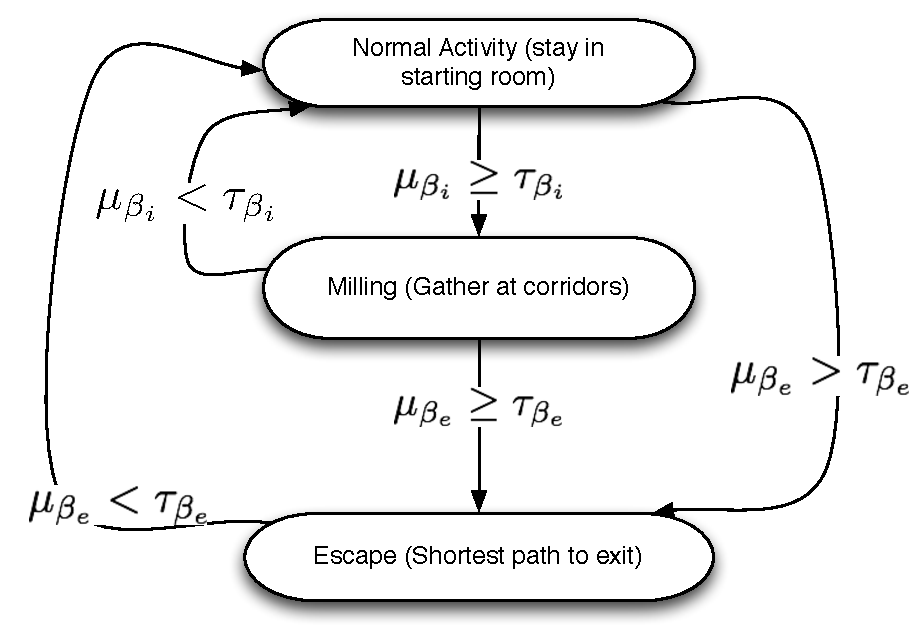
\includegraphics[width=0.65\textwidth]{EventIdentification/stateTransitions}
    \end{center}
    \caption[An illustration of the bucket model]{An illustration of the bucket model and the behavior model of agents used in the experiments. Each cue adds (or removes) a certain amount of information $\mu$ to one or both buckets ($\beta_{i}$ and $\beta_{e}$). An overfilling bucket causes a state transition.}
    \label{fig:stateTransitions}
\end{figure}

There are two sets of values here which have been mentioned: bucket thresholds ($\tau$) and the amount of information ($\mu$) that a cue contributes. As mentioned earlier, each cue is characterized by its consistency, ambiguity and source. Cues that indicate a need to egress have $\mu > 0$ and add information to buckets while cues that do not, remove information from it (i.e. $\mu<0$). Thus if an inconsistent set of cues are observed at a given time, less or maybe even no information might be added to each bucket.

The amount of information that is added or removed (i.e. the value of $\mu$) depends on the ambiguity and source of the cue. The key value in the \emph{bucket model} is the ambiguity of the cue. Each cue has an ambiguity value that is represented as a real number in the range $[0,1]$. Since each cue adds or removes information from the \emph{investigation} and \emph{egress} buckets, there are two information values associated with each cue, one for each bucket.

In theory, the amount of information added by a cue can be any decreasing function of the ambiguity of the cue. For simplicity, we assume that it is a linear function with the value added by a cue of ambiguity $\alpha$ to the bucket $\beta$ being given by:
\begin{equation}
	\mu_{\beta} (\alpha) =
    \begin{cases}

        {\tau_{\beta}}{\left[1-\frac{(\alpha^{max}_{\beta}-\alpha)}{\alpha^{max}_{\beta}}\right]}^{-1} & \mbox{ if } \alpha \leq \alpha^{max}_{\beta}\\
        0 & \mbox{ if } \alpha > \alpha^{max}_{\beta}
    \end{cases} \mbox{where } \beta \in \{\beta_{i}, \beta_{e}\}
\end{equation}

Where $\tau$ is a constant equal to the egress bucket threshold value for a normal agent and is determined by the maximum time for the bucket to fill and the intrinsic characteristics of the agent. A higher value for $\tau$ would mean more information is added per cue and the bucket would fill faster. In terms of the formula, it simply determines the slope of the curve and the range of $\mu$.  We arbitrarily choose a value $10,000$ for $\tau$ so that the rate of change of $\mu$ for every $0.1$ unit change in ambiguity $\alpha$ is greater than $1$.

$\alpha^{max}_{e}$ refers to the maximum ambiguity level that has effect on the egress bucket which in this case is fixed at $0.9$ since we assume that cues more ambiguous than this do not add any information. This helps us simulate those cues that only result in investigation even if they persist for a long time and never trigger evacuation itself. % The formula above gives the relationship shown in figure~\ref{ambiguityInfoRelationship} between ambiguity level and time to start evacuation given a single cue of that ambiguity is perceived at each second.


A similar procedure is used to determine $\mu_{i}$. An ambiguity value of $1.0$ in this case represents a small amount of information, as opposed to no information in the case of the egress bucket. This is because even an unambiguous cue when perceived for long enough initiates investigation~\cite{Tong:1985wn}. Thus, $\alpha^{max}_{i} = 1.0$.

The value for threshold of each bucket is equal to $\tau$ for normal agents. For special agents, and to consider certain special scenarios and effects, we can simply choose a threshold $\tau^s < \tau$; this will be demonstrated in the experiments in Sections~\ref{sec:experiment_2_informed_and_informing_agents},~\ref{sec:experiment_3_modelling_the_effect_of_pre_evacuation_behavior} and~\ref{sec:experiment_4}.


% Following this explain how messages contain message cues and additional information.
The effect of the source of the cue is seen in the communication model. Communication is implemented as \emph{messages} sent from one agent to the other. Each message has a message cue and environment information. The message cue works just as other cues with it's own ambiguity level. Here the term ambiguity is used to refer to the trustworthiness of the source of the information. In the current version of the model, we use a simple communication mechanism whereby agents only exchange knowledge about the state of the fire, or more precisely the inaccessible parts of the map (those blocked by fire).

In the experiments in this chapter, a simple cellular automata based fire model and a simple finite difference smoke model are used to simulate the propagation of fire and smoke\footnote{Validated models of fire and smoke are not necessary for testing the proposed model- a plausible model is sufficient}. This creates fire and smoke cues at locations near the fire which spread as the simulation proceeds. The environment itself is made up of various rooms which are connected by links. Some rooms that link multiple rooms are marked as \emph{corridors} and are the gathering points for the agents when investigating. All agents are assumed to have complete spatial knowledge of the environment and are initially located in their \emph{starting} rooms. As soon as the fire starts, fire alarm cues are placed all over the environment. Agents react to these cues and mark observable pathways that are blocked as inaccessible in their spatial knowledge graph. Agents die immediately on contact with fire. Smoke, depending on the concentration, initially slows and eventually kills agents. All agents either escape or are killed at the end of the simulation.



% To recap the discussion in Chapter~\ref{chapter:IBEVAC}, the planning system of the agent on identifying a goal passes this goal to the Navigation System that proceeds through a three-level process to determine the preferred velocity of the agent. At the highest level, a logical path is determined in terms of rooms to be crossed from the agents current location to the goal. From this logical path, spatial way points or locations are extracted by the next level. The third and final level determines a possible collision free path to the farthest visible spatial waypoint. In the experiments in this chapter, A-Star is used for path planning and RVO2 is used for the motion planning system.


% Communication between agents is also modeled with agents being able to transmit messages within a fixed communication range.




\section{Results}
\label{PreEvac:Results}

% Outline what are the things that we expect to demonstrate
This section discusses the experiments that were conducted to demonstrate the effect that cue perception, pre-evacuation behavior and communication can have on egress. The simulations were conducted on the two floor office environment shown in Figure~\ref{fig:layout}. This was adapted from the first two floors of the World Trade Center in California.  Simulations were conducted with 200 agents randomly distributed over the two floors of the building and data was collected after averaging over 20 replications of the simulation.

\begin{figure}[!tbp]
\centering
\subfloat[Ground Floor]{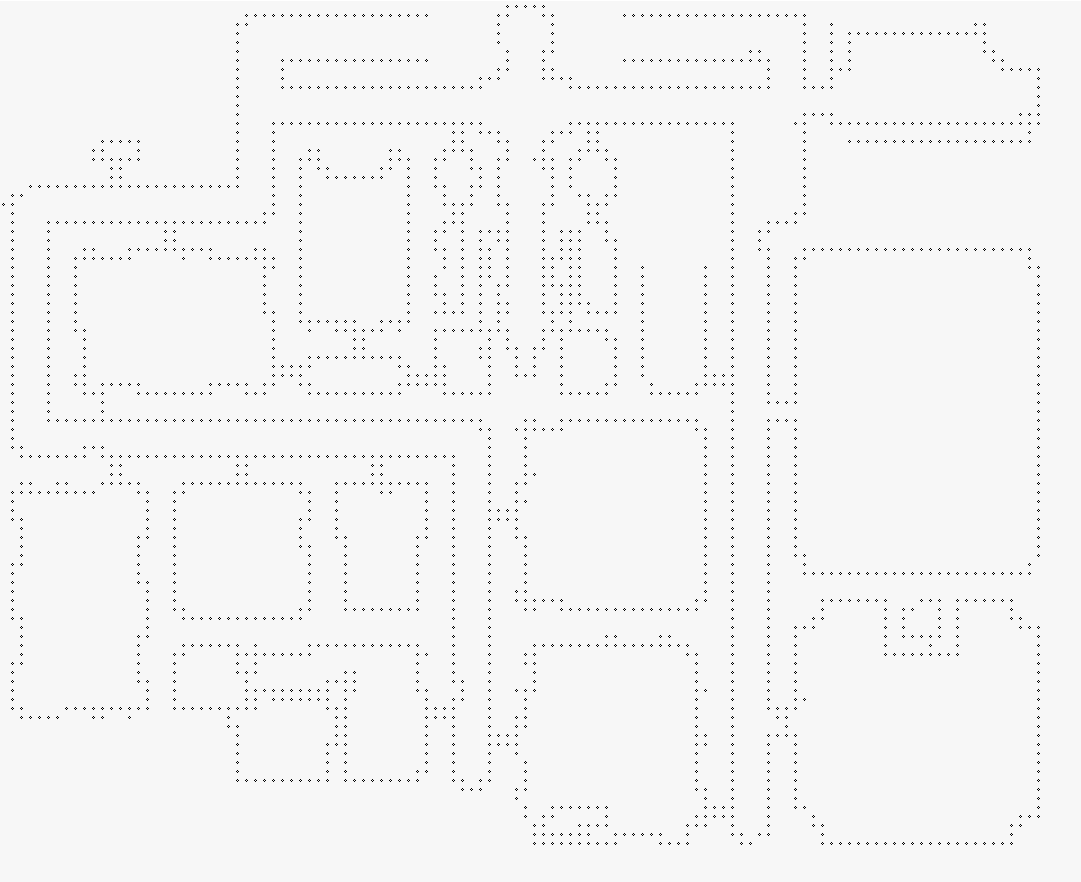
\includegraphics[width= 0.9\textwidth]{EventIdentification/floor0}}
\\
\subfloat[Second Floor]{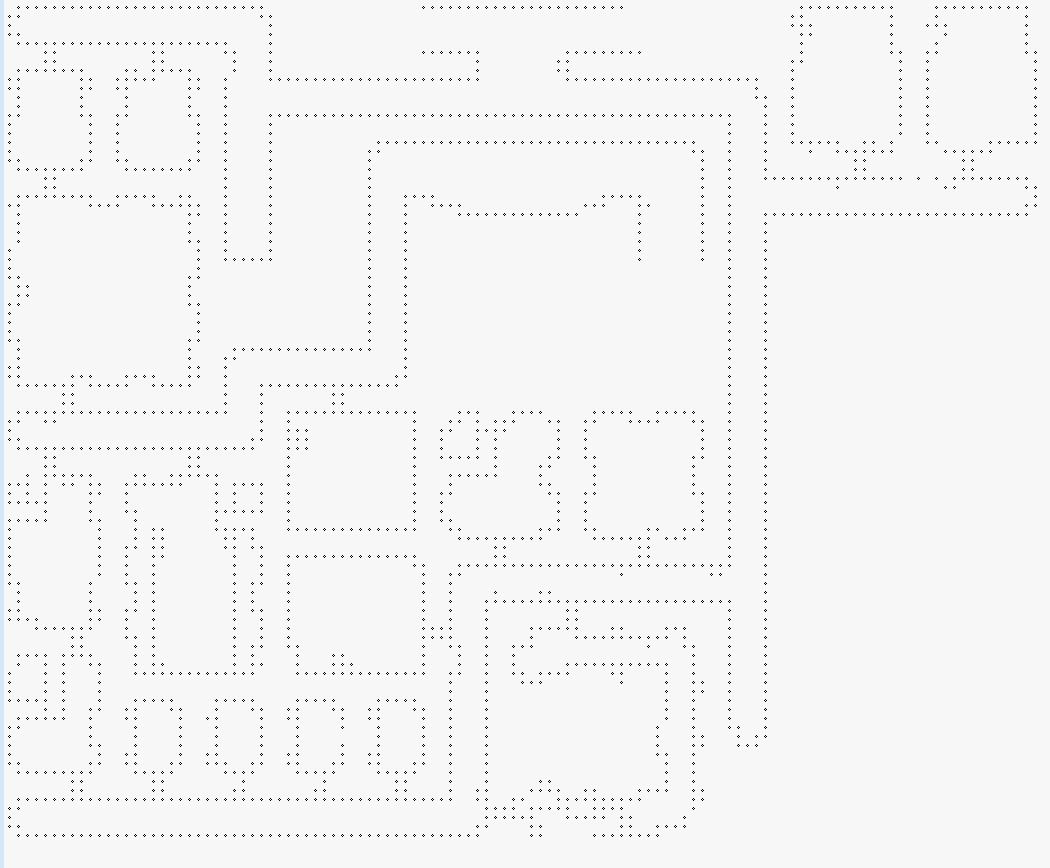
\includegraphics[width= 0.9\textwidth]{EventIdentification/floor1}}
\caption[The Environment Layout]{The two floors used for the simulation which is a modified version of the first two floors of the World Trade Center in California. The corridors, staircases and exits on both floors are marked. The numbers are the room numbers which are used in the experiments.}
\label{fig:layout}
% Change to my figure
\end{figure}

% Explain the layout of the environment, the settings and parameters

As shown in Figure~\ref{fig:layout}, the layout of the building is complex. As a result, different evacuation dynamics may be produced when the fire is started in different rooms. However, with close to a 100 rooms, running simulations with the fire starting in each room would be time consuming and, more importantly, unnecessary. Rooms close to each other or at a similar distance from the key locations (staircases and the exit) tend to produce similar dynamics. So we first grouped the rooms based on the evacuation dynamics produced in order to identify the experiments that need to be conducted. We did this by evaluating survival rates (percentage of occupants who survived) in scenarios of two types.

In the first type of scenario, we assume that all agents start evacuating immediately on hearing the fire alarm (i.e. at the start of the simulation). This is the best case scenario. Pre-evacuation behavior will increase total evacuation time and reduce survival rate. As with the other experiments, there are 200 agents randomly distributed over the two floors. Ten replications of the simulations were run for the fire starting in each room and the simulation was completed when all agents escaped or died. The survival rate was determined for each run. Figure~\ref{fig:survivalPlotRoomClassificiationImmediate} shows the results of this experiment as a heat map. The number on each room is the survival rate for that room. The standard deviation for all rooms were between $0-3$ percentage points and is not shown in the figure.
As expected, if the rooms are close to the exit or the staircase closer to the exit, then the survival rate is generally quite low. As the starting room moves further from the exit there is a higher chance of survival.


\begin{figure}[!tbp]
\centering
\subfloat[Ground Floor]{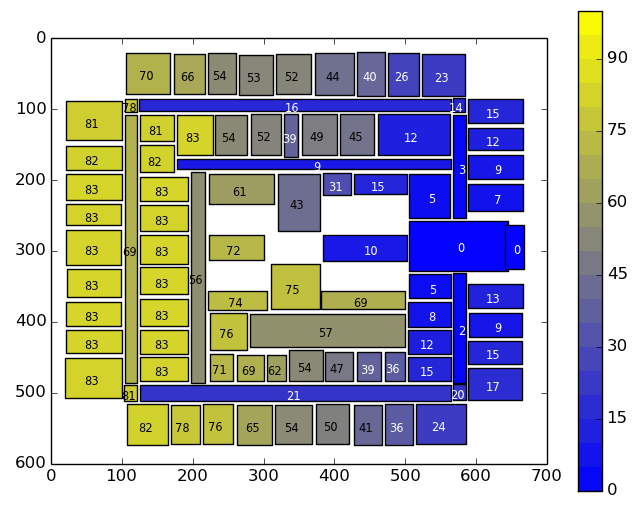
\includegraphics[width= 0.9\textwidth]{EventIdentification/heatMap-immed-floor0.PNG}}
\\
\subfloat[Second Floor]{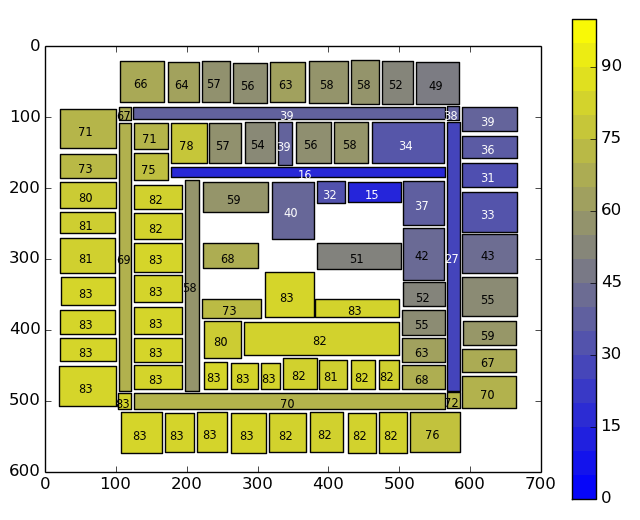
\includegraphics[width= 0.9\textwidth]{EventIdentification/heatMap-immed-floor1.PNG}}
\caption[Immediate Evacuation Survival Rate Heat Map]{This figure illustrates the survival rate when the fire is started in different rooms and evacuation starts immediately. The number on each room is the survival rate for that room.}
\label{fig:survivalPlotRoomClassificiationImmediate}
% Change to my figure
\end{figure}

There are some rooms close to the exit with lower than 40\% survival rate despite immediate evacuation. These can be ignored in our analysis, since modelling pre-evacuation behavior would not make any difference to the survival rate if the fire is started in these rooms. There are probably other rooms which can also be ignored due to the lack of effect of pre-evacuation behavior. In order to determine such groups of rooms in a more systematic manner, a second set of simulations were run with the agents only evacuating when they actually perceive the smoke (or fire). The results of this are shown in Figure~\ref{fig:survivalPlotRoomClassificationDelayed}. The pattern is mostly similar to the Figure~\ref{fig:survivalPlotRoomClassificiationImmediate} with just much lower survival rates and most survival rates being below 50\% since the occupants of a different floor generally perceive the fire/smoke too late.


\begin{figure}[!tbp]
\centering
\subfloat[Ground Floor]{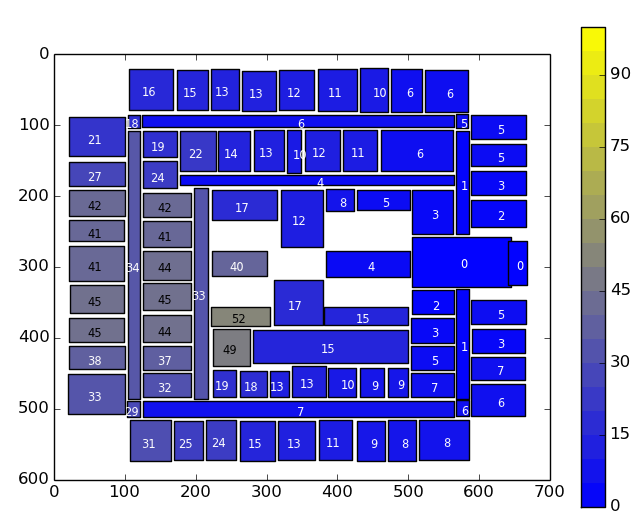
\includegraphics[width= 0.9\textwidth]{EventIdentification/heatMap-delayed-floor0.PNG}}
\\
\subfloat[Second Floor]{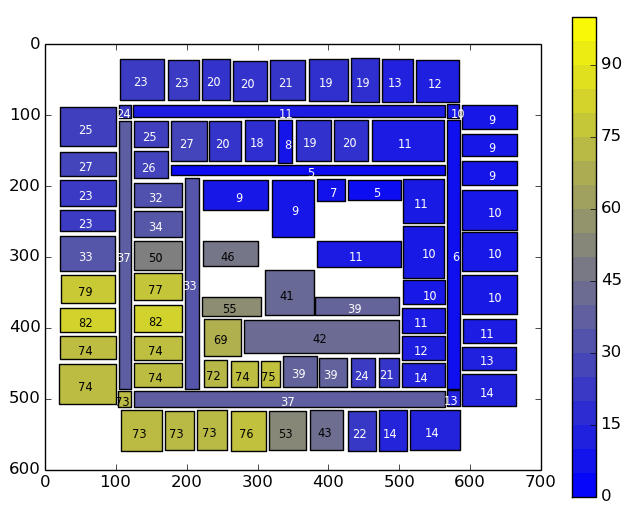
\includegraphics[width= 0.9\textwidth]{EventIdentification/heatMap-delayed-floor1.PNG}}
\caption[Delayed Evacuation Survival Rate Heat Map]{This figure illustrates the survival rate when the fire is started in different rooms and an agent starts evacuating only when it perceives the fire or smoke. The number on each room is the survival rate for that room.}
\label{fig:survivalPlotRoomClassificationDelayed}
% Change to my figure
\end{figure}


\begin{figure}[!tbp]
\centering
\subfloat[Ground Floor]{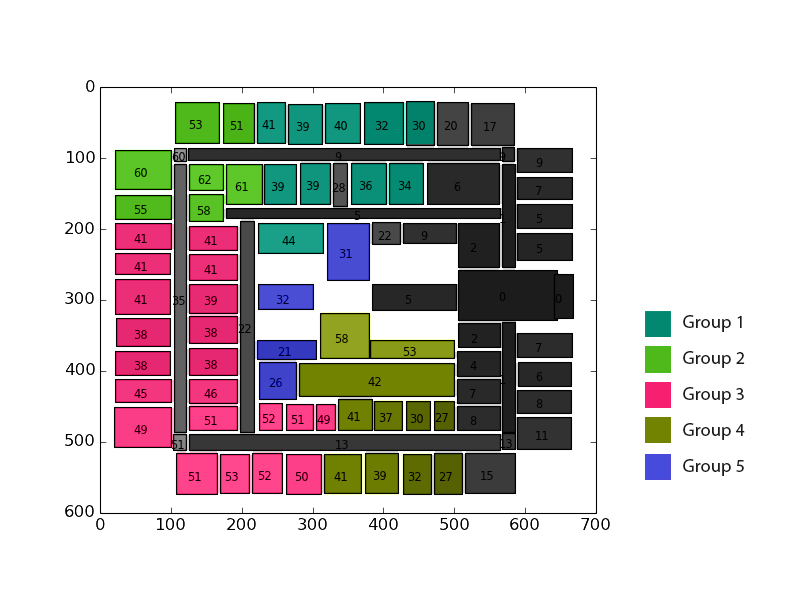
\includegraphics[width= 0.9\textwidth]{EventIdentification/heatMap-diff-floor0_GROUPED}}
\\
\subfloat[Second Floor]{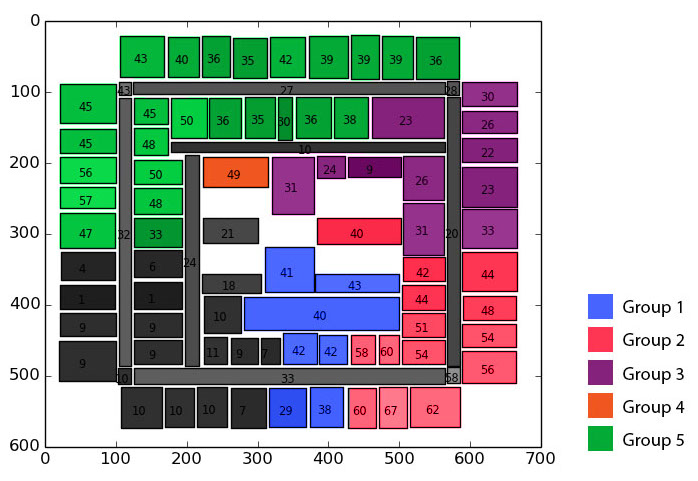
\includegraphics[width= 0.9\textwidth]{EventIdentification/heatMap-diff-floor1_GROUPED}}
\caption[Survival Rate Difference Heat Map]{This figure shows the classification of rooms into groups based on the difference in the survival rates shown in Figure~\ref{fig:survivalPlotRoomClassificiationImmediate} and Figure~\ref{fig:survivalPlotRoomClassificationDelayed}. The color of the groups are superimposed on the heat map. Corridors and rooms with very low difference are not considered to be part of any group since they are not considered in the experiments.}
\label{fig:survivalPlotRoomClassificationDiff}
% Change to my figure
\end{figure}

To understand the pattern of differences between Figure~\ref{fig:survivalPlotRoomClassificiationImmediate} and Figure~\ref{fig:survivalPlotRoomClassificationDelayed} more clearly, the difference in survival rates in the two scenarios was found and plotted in Figure~\ref{fig:survivalPlotRoomClassificationDiff}. The survival rates in this figure, along with the location of the room with respect to the two staircases and the exit to divide the rooms into 10 groups as shown in Figure~\ref{fig:survivalPlotRoomClassificationDiff}. The rooms colored black i.e. the corridors and the ones with very small differences were ignored and not used for analysis; this also includes the rooms on the bottom left corner of the second floor which was so far from the exit that most occupants inevitably survived. For each of the other groups a stereotypical room was selected which had a survival rate somewhat close the mean of the group and which was located somewhat centrally within the group. The rooms chosen for further analysis were: 14, 30, 53, 71, 81, 190, 224, 240, 252 and 377. Each of the following experiments were conducted with the fire starting in each of these rooms to understand the impact of room location on the results.



\subsection{Experiment 1: the effect of fire alarm ambiguity}
\label{PreEvac:experiment1}

A fire alarm with a simple ringing sound is much less clear and more ambiguous than a public announcement system that explicitly states that it is not a drill and gives real time updates about the situation. Thus an unambiguous fire alarm will ensure a faster evacuation and a higher survival rate. In the first experiment, we demonstrate the effectiveness of the proposed model in modelling this scenario. We make the reasonable assumption that the fire alarm can be heard clearly at every location on the map and place cues in every room.

To examine the effect of this difference in clarity of fire alarms, the experiment was repeated for different values of ambiguity (from $0.0$ - $1.0$). In this simulation, message cues are not simulated and the only other cues other than the \emph{fire alarm cues }are the \emph{fire} and \emph{smoke Cues}. A fire cue is a clear indication that there is a fire and an urgent need to start evacuation, so it is given an ambiguity of $0$. Since a smoke cue is not as clear as a fire cue we arbitrarily assign an ambiguity of $0.2$ to it.

Figure~\ref{fig:SurvivalPlotDifferentRooms} shows the percentage of agents that survived as a function of fire alarm ambiguity. As expected, regardless of the room in which the fire is started, there is a drop in number of survivors as the ambiguity of the alarm increases. This is because a less ambiguous alarm, gives more information, results in the buckets overflowing quicker, a shorter pre-evacuation period and obviously faster evacuation. A more ambiguous alarm will have to perceived for longer before it fills the bucket and triggers a state change. This delay will result in occupants further away from the exit getting insufficient time to escape depending on the room in which the fire is started. As observed earlier, the further the fire is from the exit and the staircase near the exit, the higher the survival rate.

Certain cues never trigger evacuation and, at best, trigger investigation if persisting over a period of time. In order to model this phenomenon, we explained in Section~\ref{PreEvac:EventIdentification}, how $\alpha^{max}_{e}$ is fixed at $0.9$. This means that for cues with ambiguity $\alpha > 0.9$, no information is added to the \emph{egress bucket} $\beta_{e}$.
This results in the sharp drop at $\alpha = 1.0$ in Figure~\ref{fig:SurvivalPlotDifferentRooms} as agents only start evacuating when they actually observe the fire or smoke cues themselves. Even in this scenario, however, the survival rate is higher than shown in Figure~\ref{fig:survivalPlotRoomClassificationDelayed} because milling behavior still takes place. The effect of milling is analyzed in more detail in Section~\ref{sec:experiment_3_modelling_the_effect_of_pre_evacuation_behavior}.

The flat curve for room number 252 is interesting but not surprising. This is because of the peculiar location of the room far from both staircases and on the second floor. Thus, for any value of $\alpha < 0.9$, most evacuees have enough time to escape before the fire and smoke blocks the crucial staircases and exits. For $\alpha > 0.9$ however, as explained previously, egress does not start until the smoke or fire is directly perceived and results in a sharp drop in survival rate.

\begin{figure}[!t]
	\centering
		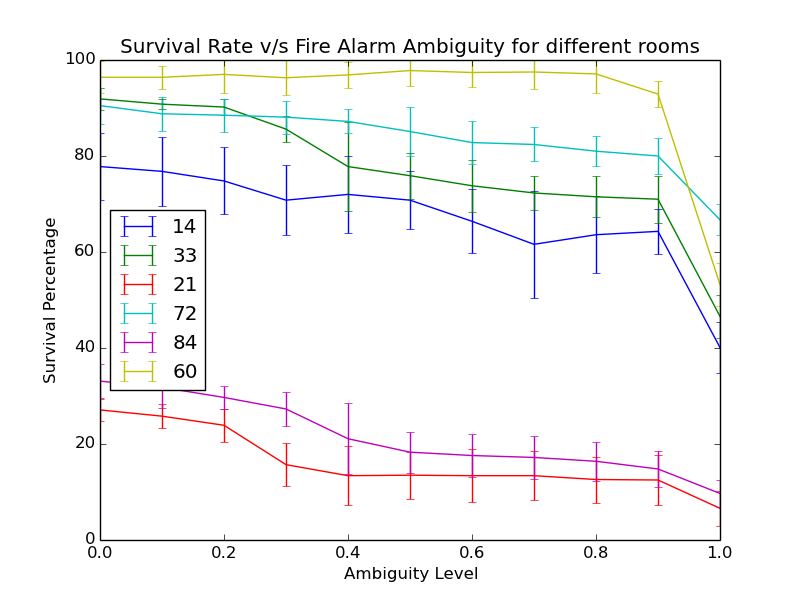
\includegraphics[width=0.95\textwidth]{EventIdentification/survivalPlotFireAlarmDifferentRooms.png}

	\caption[Experiment 1: The effect of fire alarm ambiguity]{This figure shows the percentage of evacuees that survived as a function of the ambiguity with the fire being started in different rooms. While there are obvious inter room differences, it can be clearly seen that the more ambiguous an alarm, the lower the survival rate.}
	\label{fig:SurvivalPlotDifferentRooms}
\end{figure}

This experiment has highlighted the importance of modelling and considering pre-evacuation behavior and the value of having a clear and unambiguous fire alarm. While, the effect of ambiguity of fire alarm and pre-evacuation is clearly seen independent of the location of the fire, the location does affect the extent of this effect.




\subsection{Experiment 2: informed and informing agents} % (fold)
\label{sec:experiment_2_informed_and_informing_agents}

In a situation where it is possible to inform a certain number of occupants of a building about the urgent need to evacuate and these occupants inform others as they evacuate, an interesting question might be to examine how many people need to be informed for this strategy to be effective. To examine this, we divide the set of agents into two groups:  normal agents and informed agents. The former behaves as in the previous; the latter start evacuating as soon as the simulation starts and broadcast messages to other agents to start evacuating immediately. This immediate evacuation can be modeled by setting the threshold of both the investigation and the egress bucket to zero thus ensuring that the phase is triggered right after the first time-step of the simulation. Message cues that have an informed agent as their source have an ambiguity of 0 indicating that these messages are completely trusted by other agents. The fire alarm ambiguity cue is set to $1.0$ to minimize it's effect.

Simulations were conducted with the proportion of informed agents varied from 10\% to 100\% of the 200 agents. Experiments were run with the fire starting in each of the stereotypical rooms. The blue curve in Figures~\ref{fig:informed14}, \ref{fig:informed30}, \ref{fig:informed53}, \ref{fig:informed71}, \ref{fig:informed81}, \ref{fig:informed190}, \ref{fig:informed224}, \ref{fig:informed240}, \ref{fig:informed252} and \ref{fig:informed377} shows the results of this experiment.

\begin{figure}[!t]
\centering
        \subfloat[Room 14]{\label{fig:informed14}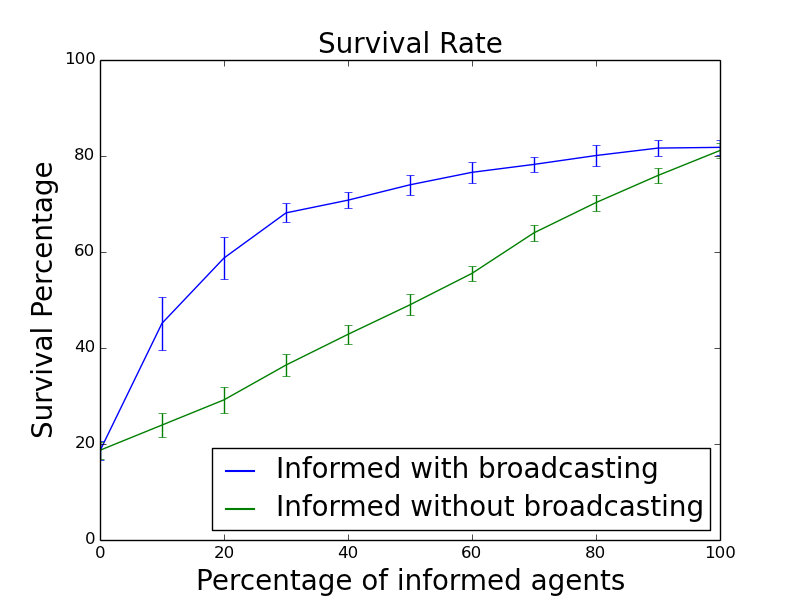
\includegraphics[width= 0.48\textwidth]{EventIdentification/14-informedVSInforming}}
    \hspace{1pt}
        \subfloat[Room 30]{\label{fig:informed30}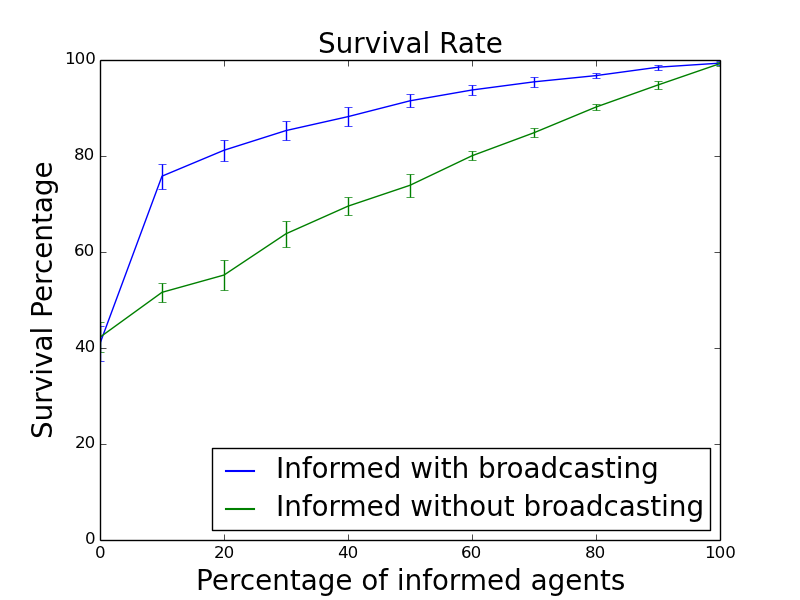
\includegraphics[width= 0.48\textwidth]{EventIdentification/30-informedVSInforming}}
    \\
        \subfloat[Room 53]{\label{fig:informed53}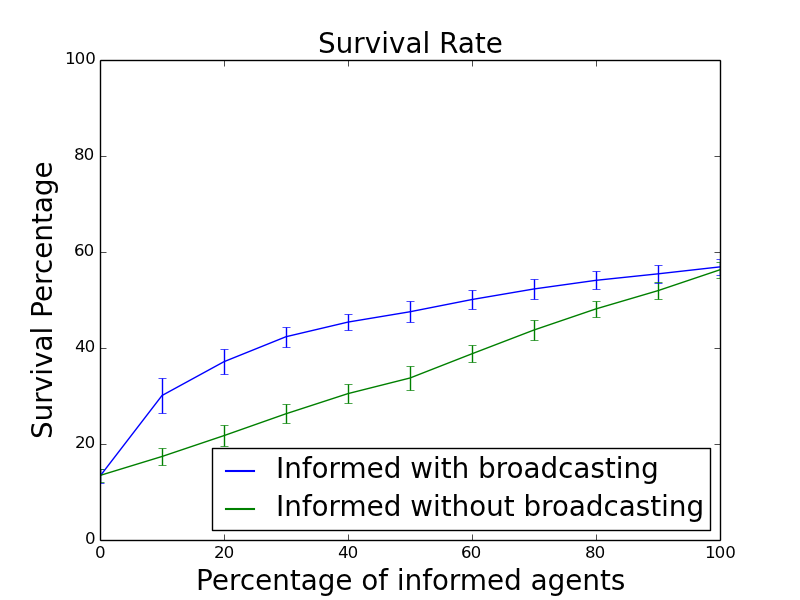
\includegraphics[width= 0.48\textwidth]{EventIdentification/53-informedVSInforming}}
    \hspace{1pt}
        \subfloat[Room 71]{\label{fig:informed71}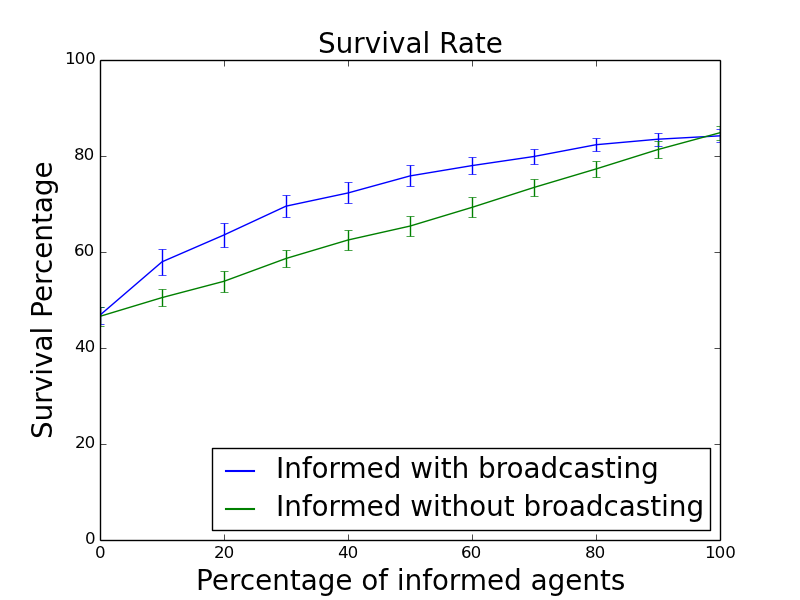
\includegraphics[width= 0.48\textwidth]{EventIdentification/71-informedVSInforming}}
    \\
        \subfloat[Room 81]{\label{fig:informed81}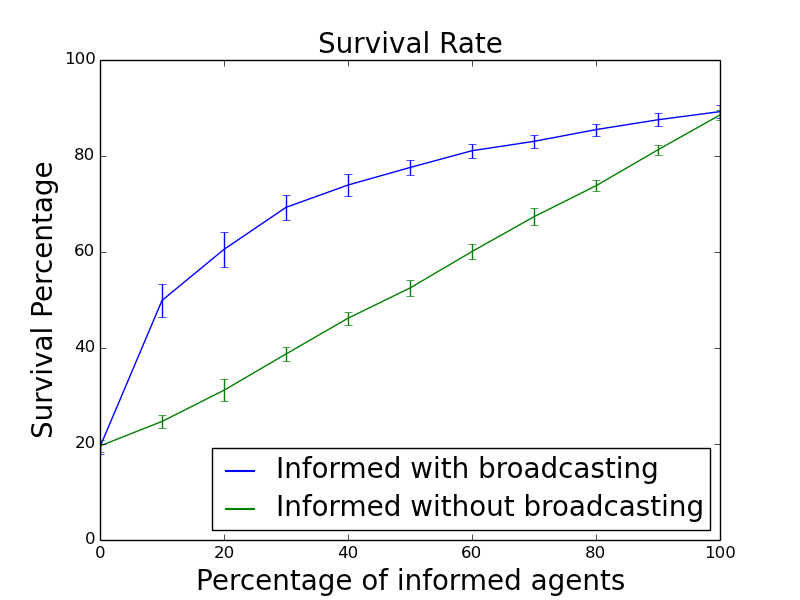
\includegraphics[width= 0.48\textwidth]{EventIdentification/81-informedVSInforming}}
    \hspace{1pt}
        \subfloat[Room 190]{\label{fig:informed190}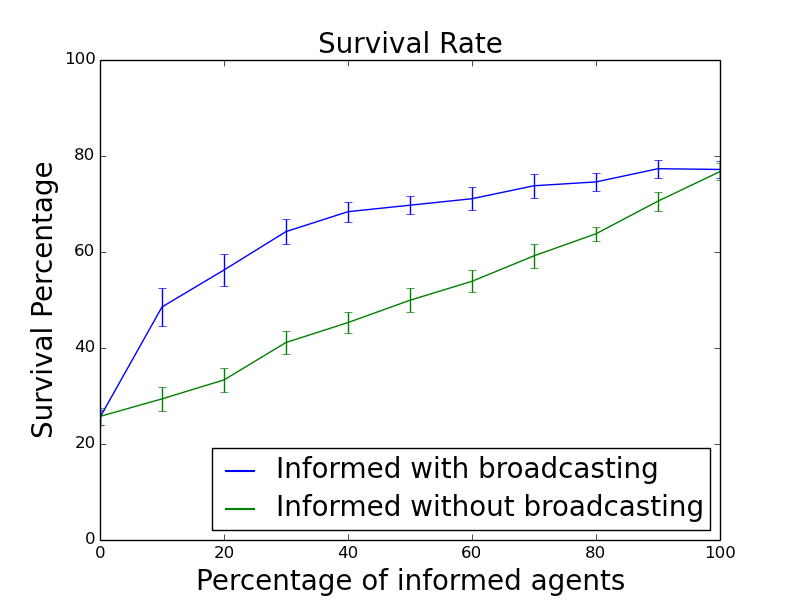
\includegraphics[width= 0.48\textwidth]{EventIdentification/190-informedVSInforming}}
    \caption[Experiment 2: The effect of having informed occupants]{These figures show the effect of informing a certain set of agents to evacuate immediately. The blue curve shows the survival rate when these informed agents broadcast and inform other agents as they evacuate. The other curve helps contrast this with the situation where the informed agents simply evacuate without informing other agents, thus illustrating the importance that informed agents also inform others as the evacuate.}
    \label{fig:informed_vs_informing_1}
\end{figure}

\begin{figure}[!t]
\centering
        \subfloat[Room 224]{\label{fig:informed224}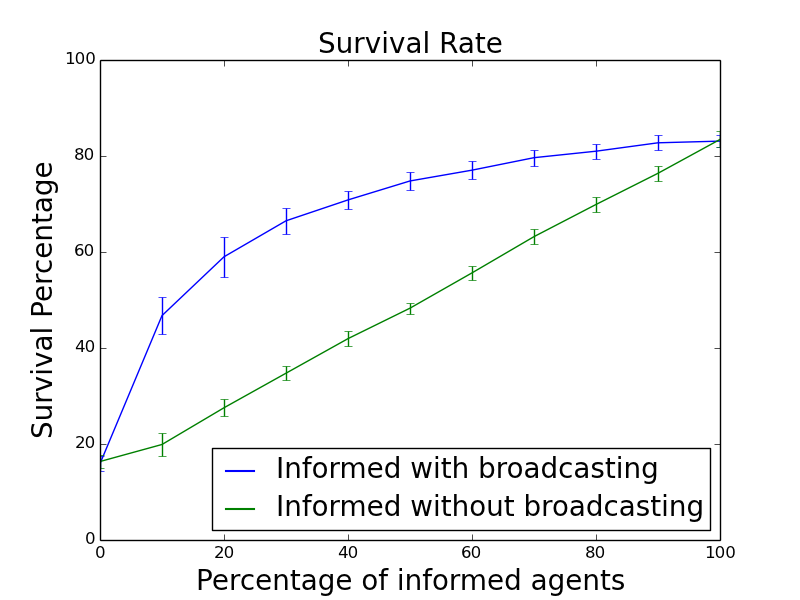
\includegraphics[width= 0.48\textwidth]{EventIdentification/224-informedVSInforming}}
    \hspace{1pt}
        \subfloat[Room 240]{\label{fig:informed240}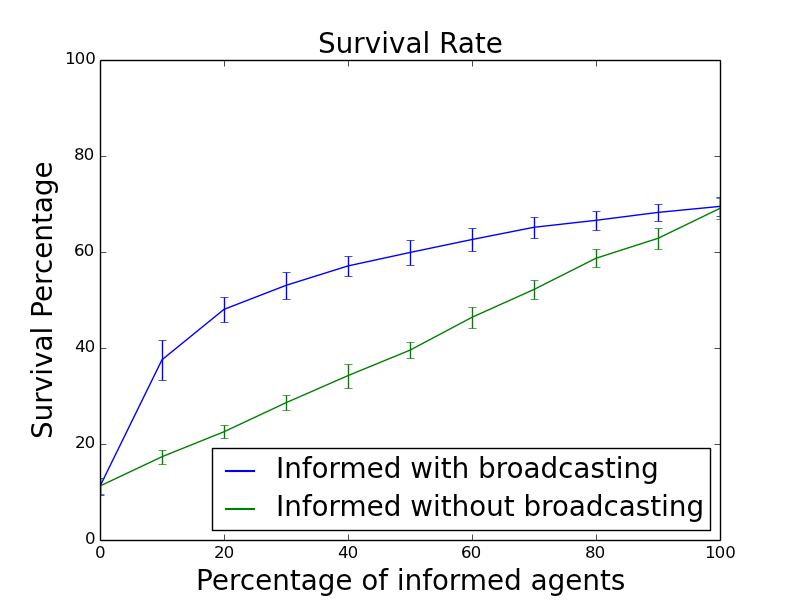
\includegraphics[width= 0.48\textwidth]{EventIdentification/240-informedVSInforming}}
    \\
        \subfloat[Room 252]{\label{fig:informed252}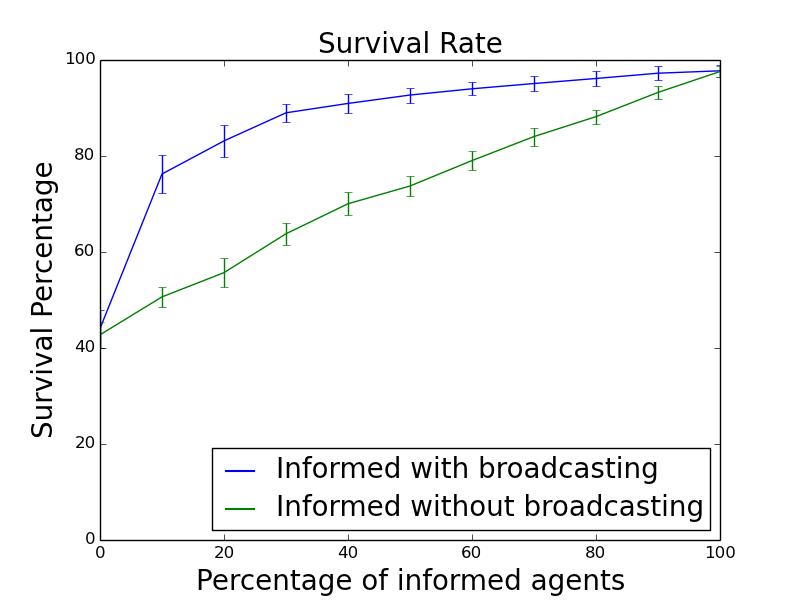
\includegraphics[width= 0.48\textwidth]{EventIdentification/252-informedVSInforming}}
    \hspace{1pt}
        \subfloat[Room 377]{\label{fig:informed377}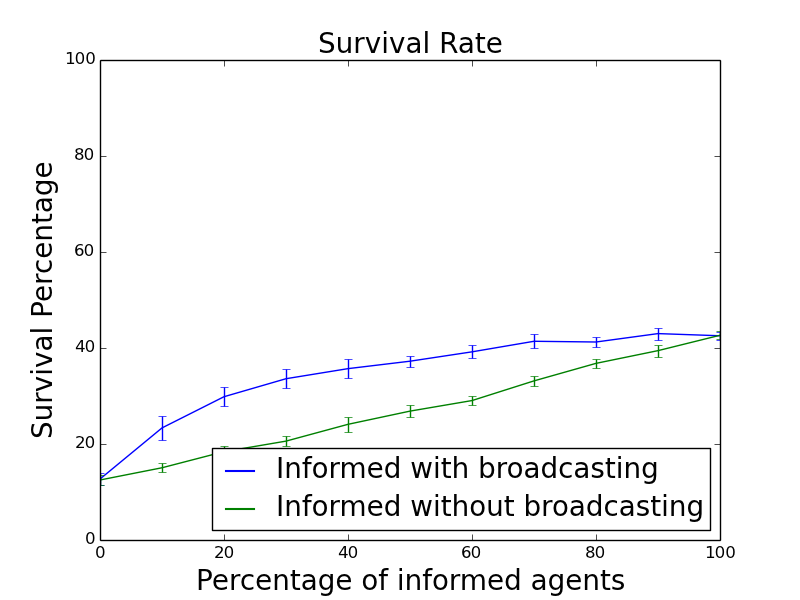
\includegraphics[width= 0.48\textwidth]{EventIdentification/377-informedVSInforming}}
    \caption[Experiment 2: The effect of having informed occupants (contd.)]{These figures show the effect of informing a certain set of agents to evacuate immediately. The blue curve shows the survival rate when these informed agents broadcast and inform other agents as they evacuate. The other curve helps contrast this with the situation where the informed agents simply evacuate without informing other agents, thus illustrating the importance that informed agents also inform others as the evacuate. (contd.)}
    \label{fig:informed_vs_informing_2}
\end{figure}

Except in the case of the fire starting in room 377, with just 15\% agents being informed the survival rate increased two fold or three fold in almost all cases. Room 377 being so close the vital staircase that is close to the exit, has less than 50\% survival regardless of the situation (As also seen in Figure~\ref{fig:survivalPlotRoomClassificiationImmediate} and Figure~\ref{fig:SurvivalPlotDifferentRooms}) and expectedly shows a much slower rate of improvement than the other rooms. Also except in the cases where the fire starts in room 377 and 53, survival rate is greater than 50\% and, in most cases, greater than 60\% with just 20\% of the occupants being informed.

In order to isolate the effect of these informed agents propagating information, the red curve in the Figures~\ref{fig:informed_vs_informing_1} and~\ref{fig:informed_vs_informing_2}  shows the effect of these agents only being \emph{informed} agents that evacuate immediately without \emph{informing} other agents. The importance of these evacuating agents broadcasting the information they know is highlighted by the 20-30\% difference in survival rates that are observed when 20-60\% of the occupants are informed. This difference is lesser but still significant even in the case of room 377, 53 and 71. What is common to these rooms are their proximity to the staircase closer to the exit. This is probably because when this staircase is blocked the shortest route towards the exit becomes longer. This results in more deaths.

This section demonstrated the usefulness of informing and possibly training a certain proportion of the agents about the need to evacuate. Even when randomly distributed in the environment, less than a quarter of the occupants of a building need to be trained for significant improvements to be observed. More strategic placement of the informed occupants would obviously mean fewer of them are required. The usefulness of strategic placement of informed occupants is considered in more detail in Section~\ref{sec:experiment_4}.

The experiments also revealed the importance of these informed occupants broadcasting their knowledge as they escape. Again, the scenario tested in this experiment was quite simple in the sense that these informed agents informed only those occupants that it met while moving towards the exit. Their effectiveness will probably be much higher if they actively tried to inform other agents. However, in that situation, there is the added consideration of how much effort should they make in finding and informing others before making their own way to the exit. However, one of the reasons for the effectiveness of these informed agents is that most of the uninformed occupants would have been \emph{milling} in the corridors and were thus easily reachable; this probably alleviates the need for the informing agents to actively try and find and inform other agents. In the next experiments, we examine the importance of this milling behavior.



% section experiment_3_informed_and_informing_agents (end)

\subsection{Experiment 3: is milling important?} % (fold)
\label{sec:experiment_3_modelling_the_effect_of_pre_evacuation_behavior}

The milling effect of people gathering in a common location to investigate and confirm the need to evacuate has been reported by interviewers of victims~\cite{Fahy:2010to,Purser:2001ts} and is also one of the main features of the evacuation behavior modeled in this chapter. However, it is also a feature that is generally ignored in most models. Even in the rare cases that do consider pre-evacuation behavior, it is simply modeled as delay in evacuation. In this section, the importance of modelling milling behavior is demonstrated.

For this experiment, we compare agents that mill against agents that don't mill and simply move straight to evacuation. We model this by creating a new kind of agent that has an investigation threshold $\tau_{beta_{i}}= +\infty$ is modeled. These agents will have their egress bucket $\beta_{e}$ overflowing before their investigation bucket $\beta_{i}$. Thus, they transition straight from normal behavior to evacuation (Figure~\ref{fig:stateTransitions}). We compare these agents against the original agents to test the hypothesis that milling behavior has a significant effect on evacuation characteristics. Since both agents have the same threshold for the egress bucket they will both start evacuating at the same time and the normal evacuation characteristics are identical.

Milling is important and useful in situations where evacuees communicate with each other. So, in the first experiment we fix the message ambiguity as 0.0 and fix fire alarm ambiguity at 1.0 so that agents only start evacuating, either if they see the actual fire or smoke or if they are told about the fire by evacuating agents. We only do the analysis on agents spawned in the first floor because the agents in the second floor have no way of knowing about the need for evacuation until it's too late. Figure~\ref{fig:MillingSurvivalPlot} compares the survival rates with milling against the situation where there is only delayed evacuation. The figure clearly shows milling improves survival rate in all but the two cases where the fire is started in rooms 190 and 224. In these situations the fire is farthest from the staircases and the exits. Thus, most agents on the higher floors escape by the shortest route i.e. the staircase near the top right. This also means that they avoid most occupants of the first floor who get trapped without knowing about the fire.

% This difference is much more clearly illustrated when we plot the average time at which the last agent starts evacuating in both situations shown in figure~\ref{fig:MillingLastPerson}.


\begin{figure}[!t]
	\begin{center}
		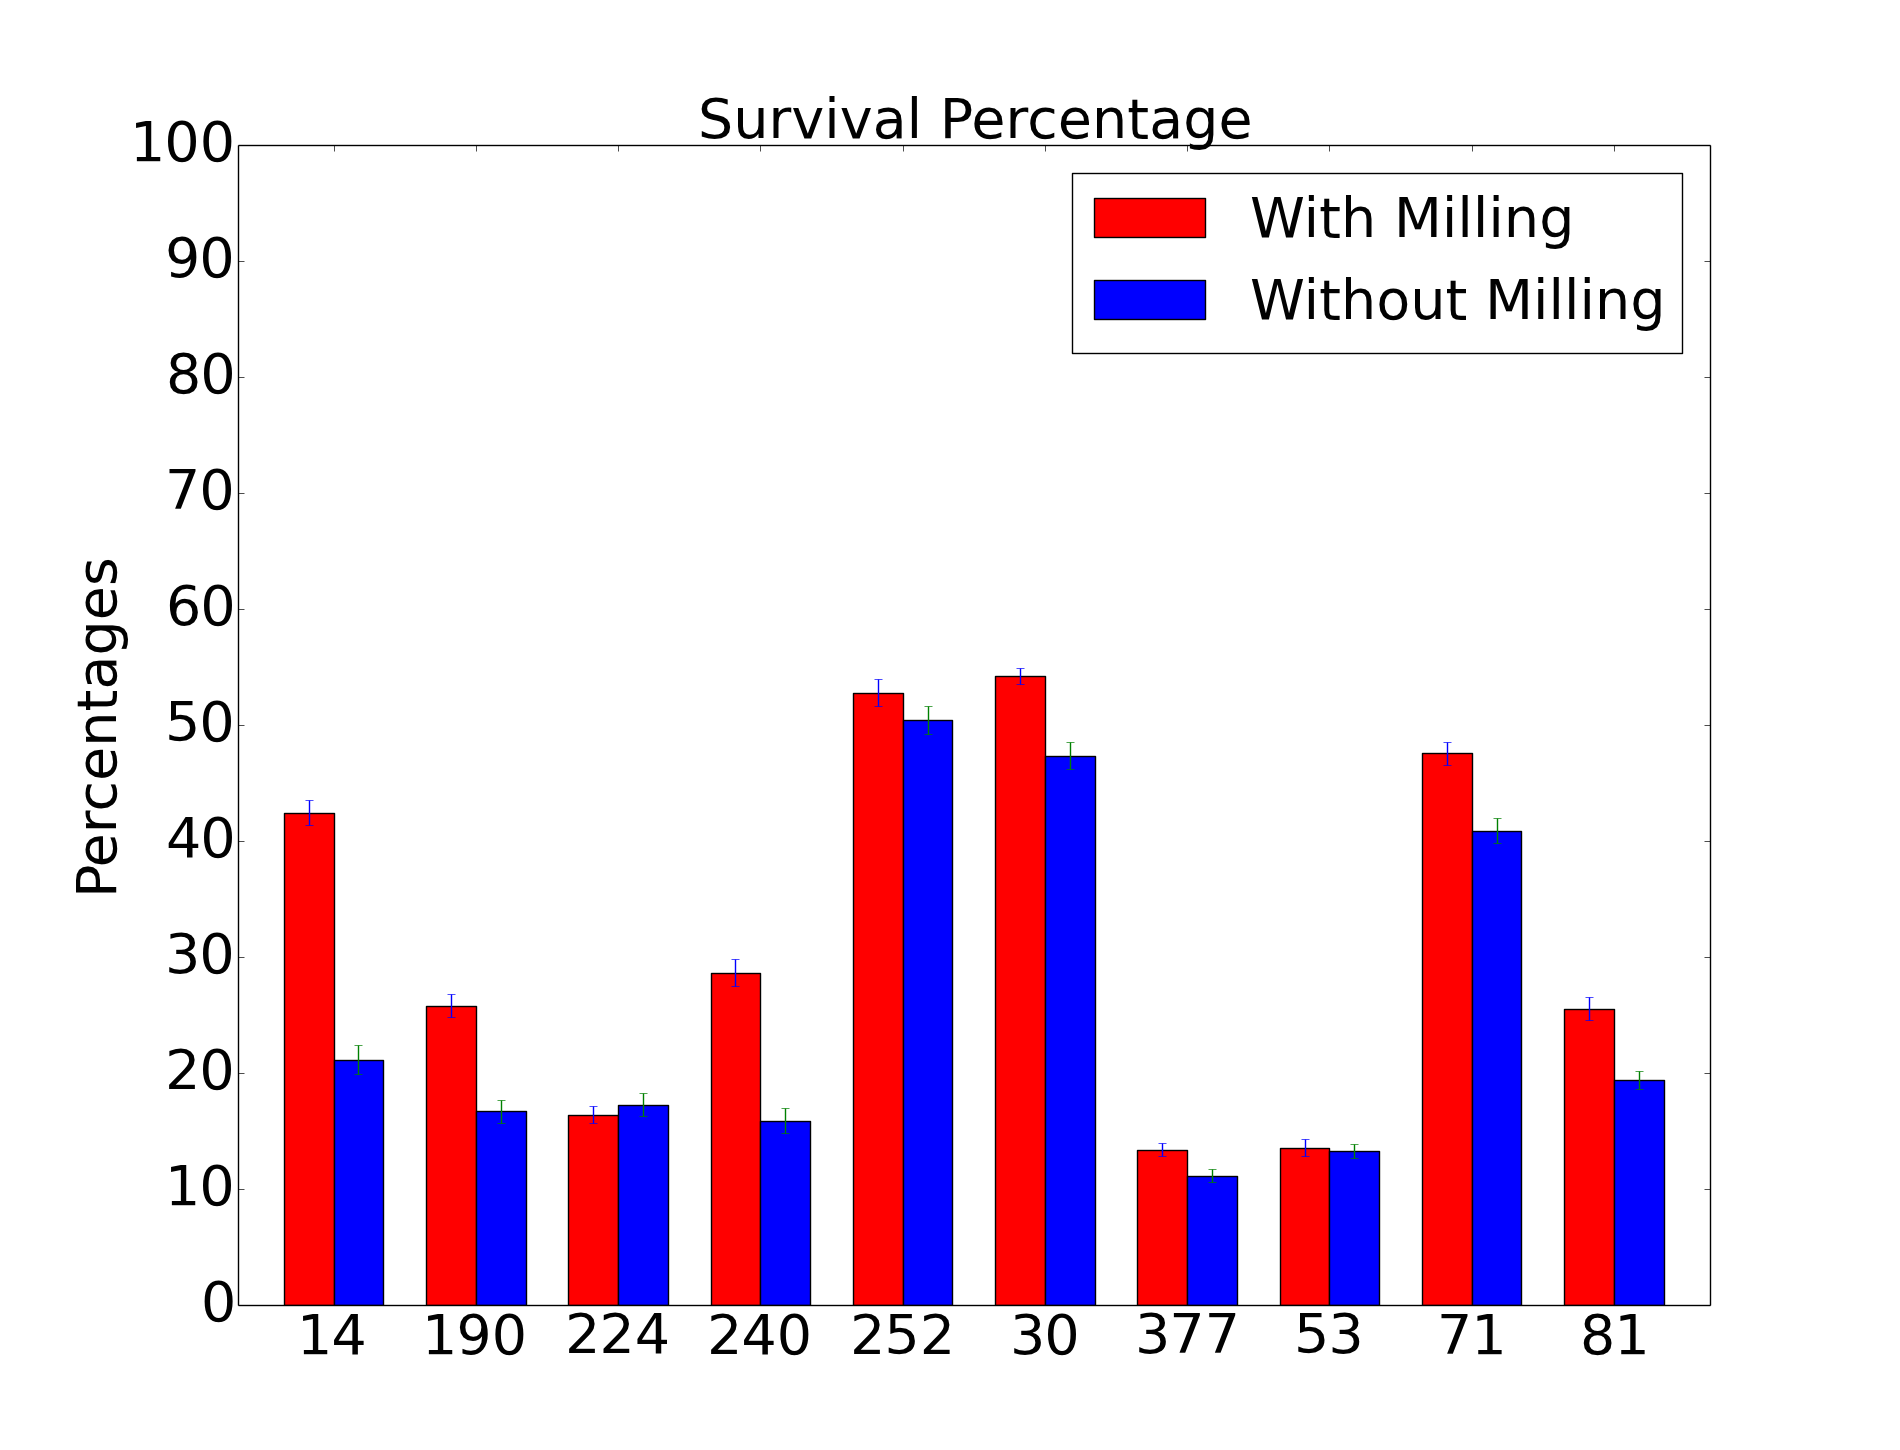
\includegraphics[width=\textwidth]{EventIdentification/millingSurvivalPlot}
	\end{center}
	\caption[Experiment 3: The importance of milling]{The figure illustrates the difference created by and the usefulness of milling behavior by showing the increase in survival rate that is observed when there is milling against when there isn't milling/ pre-evacuation behavior.}
	\label{fig:MillingSurvivalPlot}
\end{figure}
% section experiment_3_the_importance_of_spatial_knowledge_propagation (end)

\subsection{Experiment 4: the importance of spatial knowledge propagation} % (fold)
\label{sec:experiment_4}



In experiment 2, we considered the effect of having a certain proportion of the occupants as trained personnel who are informed immediately about the need to evacuate. A simplistic scenario where these informed agents are randomly distributed over the environment was modeled and their effectiveness demonstrated. Significant improvement was seen because the evacuating informed agents not only informed other agents about the need to evacuate but also transmitted information about the areas that they knew were inaccessible. This is a significant advantage that a set of trained/ informed personnel can have over the most expensive or unambiguous fire alarm. Unambiguous fire alarms like loudspeakers or PA systems constantly giving instructions would still find it very difficult to transmit spatial information. Thus despite getting everyone informed and evacuating, no one would know where the fire is. In this experiment, we test whether spatial knowledge propagation through informed personnel can be an improvement over an unambiguous fire alarm.

The informed agents we consider in this experiment are different from those in Experiment 2 in two ways. Firstly, informed agents are modeled such that they can communicate spatial and cue information to other informed agents immediately. This is a reasonable assumption since it is likely that trained personnel will have some method for communicating efficiently with each other. Secondly, rather than being randomly distributed over the environment, they are located such that each corridor has one informed agent. This strategic distribution increases the likelihood that at least one informed agent perceives the fire and knows its location and propagates this information across the informed agent network.

The usefulness of spatial knowledge propagation would be best seen in a situation where survival rate is low due lack of spatial knowledge. Thus, we chose room 53 as starting point of the fire based on the results of the fire alarm ambiguity experiment (Figure~\ref{fig:SurvivalPlotDifferentRooms}). An empirical observation of the simulation of this scenario  confirmed that one of the major reasons for dropping survival rate was the lack of spatial knowledge. Evacuees would realize too late that the staircase close the exit was blocked and would not have enough time to reroute and escape. Figure~\ref{fig:tannoyExperiment} illustrates the result of running 20 replications of the scenario with strategically distributed informed agents and contrasts this with a situation without these agents.

\begin{figure}[!t]
    \centering
    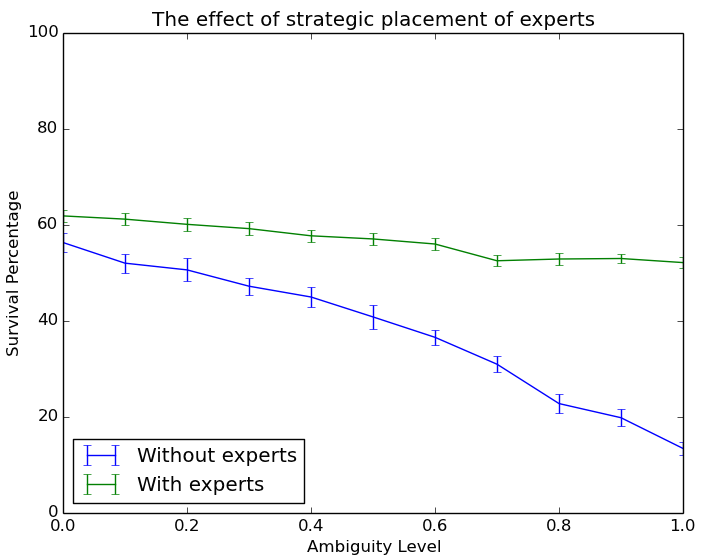
\includegraphics[width=\textwidth]{EventIdentification/tannoyExperiment}
    \caption[Experiment 4: The importance of spatial knowledge propagation]{Simulation results indicate that strategically placed informed agents can provide a significant improvement in evacuation efficiency and is as effective as an unambiguous fire alarm in ensuring higher survival rate.}
    \label{fig:tannoyExperiment}
\end{figure}

The simulation results seem to indicate that in scenarios like this, informed agents do indeed make a difference. Close to 60\% survival rate is observed in scenarios with informed agents regardless of the ambiguity of the alarm while normally survival rate would fall to below 20\%. More interestingly, there seems to be some improvement in survival rate even when compared against an unambiguous fire alarm. In fact, even in situations with a highly ambiguous fire alarm, strategically placed informed agents seem to have as much effectiveness as an unambiguous fire alarm would have.

% section experiment_4_modelling_the_effect_of_pre_evacuation_behavior (end)
\section{Conclusion and Future Work}
\label{PreEvac:ConclusionAndFutureWork}

This chapter began with a discussion of the need to model pre-evacuation behavior. A novel cue modelling and perception system which enables the detailed modelling of pre-evacuation behavior was then described. This model is based on the work of Kuligowski~\cite{Kuligowski:2009un} and is based on the idea of perceived cues adding information to two information buckets whose overflowing results in phase changes. Occupants first start an investigation phase and once the need for evacuation is confirmed, they start evacuating. It was demonstrated through simulation that modelling pre-evacuation behavior and the effect of ambiguity of perceived cues can have significant effects on evacuation dynamics and efficiency. The value of training a certain proportion of the population and the critical number of these trained personnel needed was identified. Simulations indicate that strategic placement and training of a small subset of occupants might be cheaper but just as effective as an expensive and unambiguous fire alarm. The value of milling behavior and the need for modelling this was also demonstrated through simulations.

The proposed pre-evacuation behavior model can be a valuable tool for studying and analyzing many more real world issues. Similar simulations can be used to do safety by design analysis of buildings by ensuring that milling/gathering points are efficiently located. Other safety-by-design elements might have to do with budget constraints during large events or festivals. Strategic placement of more expensive but less ambiguous fire alarms along with some cheaper more ambiguous ones can reduce the cost while ensuring the effectiveness of emergency systems during these events.

While the model is based on theories that are based on studies of real world incidents, the results produced have not been validated against real world data. In the absence of detailed video footage or at least statistics of people evacuating from a building, validating a model of pre-evacuation behavior is very difficult. This is especially so, because in fire-drills and practices the observed pre-evacuation dynamics will be very different because the evacuees generally have prior knowledge of the drill.

Setting up a controlled experiment is difficult due to the dangers involved to participants. A possible way to tackle this difficulty in getting real world data would be to make use of virtual environments like games. This could be used
to improve our understanding of cues and their effect on pre-evacuation behavior in general. We explore this approach further in the next chapter where a game based approach is used for studying human exploration behavior.


In the simulations in this chapter it was assumed that each agent had complete knowledge of the environment, at least in terms of every room and how to get to each room. This is almost never the situation in the real world and to improve the efficacy of simulations it is necessary to model this partial knowledge. However, our current understanding of how people explore a partially known environment and how their knowledge develops over time are both very limited. The next chapter presents a game based methodology for studying this.
